\newpage
\subsection{Actividad 13}
Diseñar un controlador analógico tipo PID (PD, PI, PID) para el
sistema servomotor de posición por el \textsc{método de
Ziegler-Nichols} en abierto y cerrado (si son posibles) y realizar su
discretizacion con $T=0.05$ aplicando el método trapezoidal y graficar
la respuesta escalón unitaria del sistema de control en bucle cerrado
del servomotor de posición a través de la herramienta \textsc{rltool}.

Para implementar el método Ziegler-Nichols en bucle abierto,
necesitamos que la respuesta ante entrada escalón sea aproximadamente
la de un sistema de primer orden con retardo, por lo que no podemos
aplicar este método.  Por el contrario sí podemos implementar el
método Ziegler-Nichols en bucle cerrado.

\begin{tcolorbox}[sharp corners, colframe=bluebox, title= Método de
Ziegler-Nichols, breakable=unlimited]
 $>>>$ step(Gposicion)
  \vspace*{0.35em}
  \mkanscode{
\begin{figure}[H]
  \centering
  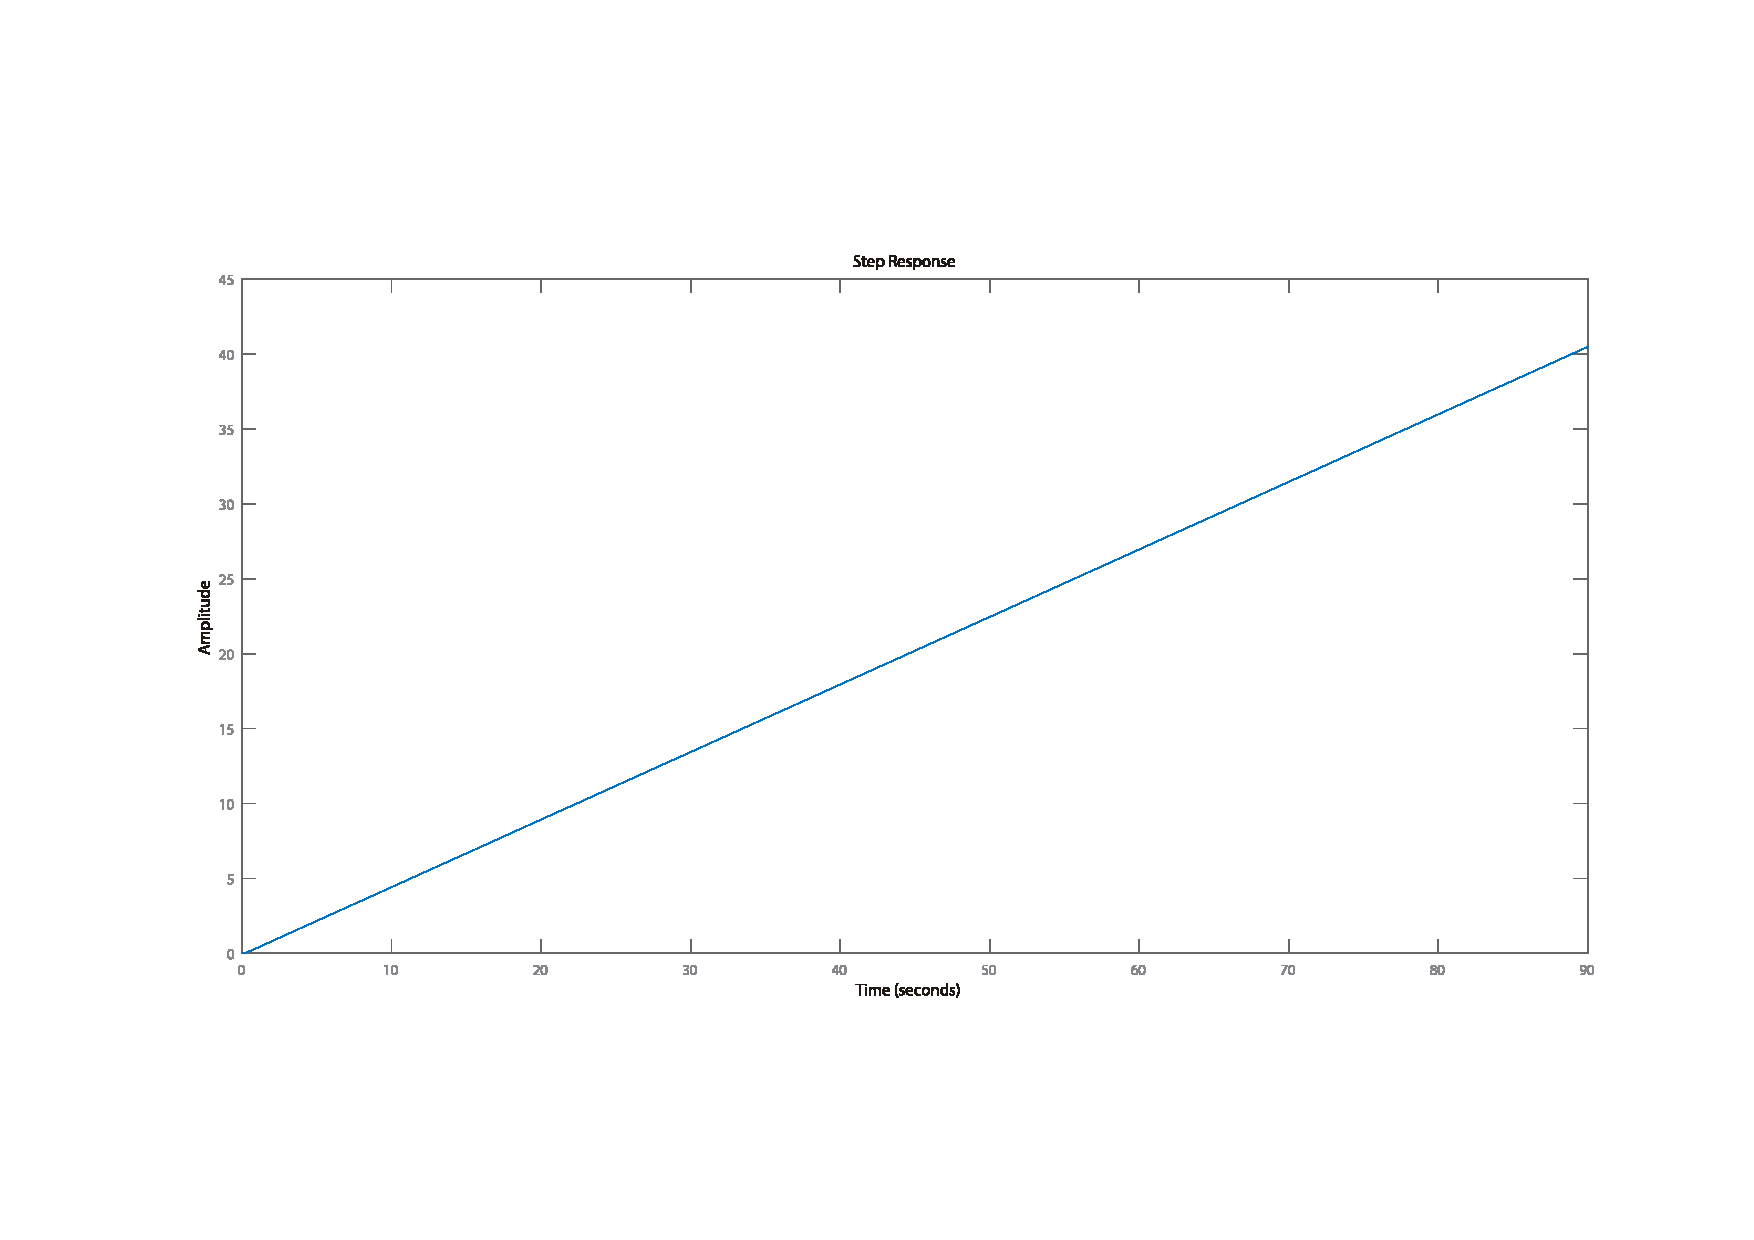
\includegraphics[clip, trim=2cm 3.6cm 1.4cm 3.4cm,scale=0.48]{images/figura 22.pdf}
  % izquierda,abajo,derecha,arriba
  \caption{Respuesta del sistema en bucle abierto frente a un escalón.}
    \label{fig:figura 22}
\end{figure}
}

Como es inestable no se puede hacer el PID Ziegler-Nichols en bucle
abierto, por lo tanto lo haremos en bucle cerrado.

$>>>$ [Kc,Pm,Wg]=margin(kr*Gposicion);\\
$>>>$ Tc = 2*pi/Wg;\\
$>>>$ Kp = 0.75*Kc;\\
$>>>$ Ti = Tc/1.6;\\
$>>>$ Ki = Kp/Ti;\\
$>>>$ Td = Tc/10;\\
$>>>$ Kd = Td*Kp;\\
$>>>$ tf = 0.01;\\
$>>>$ pidZN = pid(Kp,Ki,Kd,tf);\\
$>>>$ rltool(Gposicion,pidZN);\\
$>>>$ pidZNz = c2d(pidZN,T,'trapezoidal');\\
$>>>$ rltool(Gposicionz,pidZNz);\\

  \vspace*{0.35em}
  \mkanscode{
\begin{figure}[H]
  \centering
  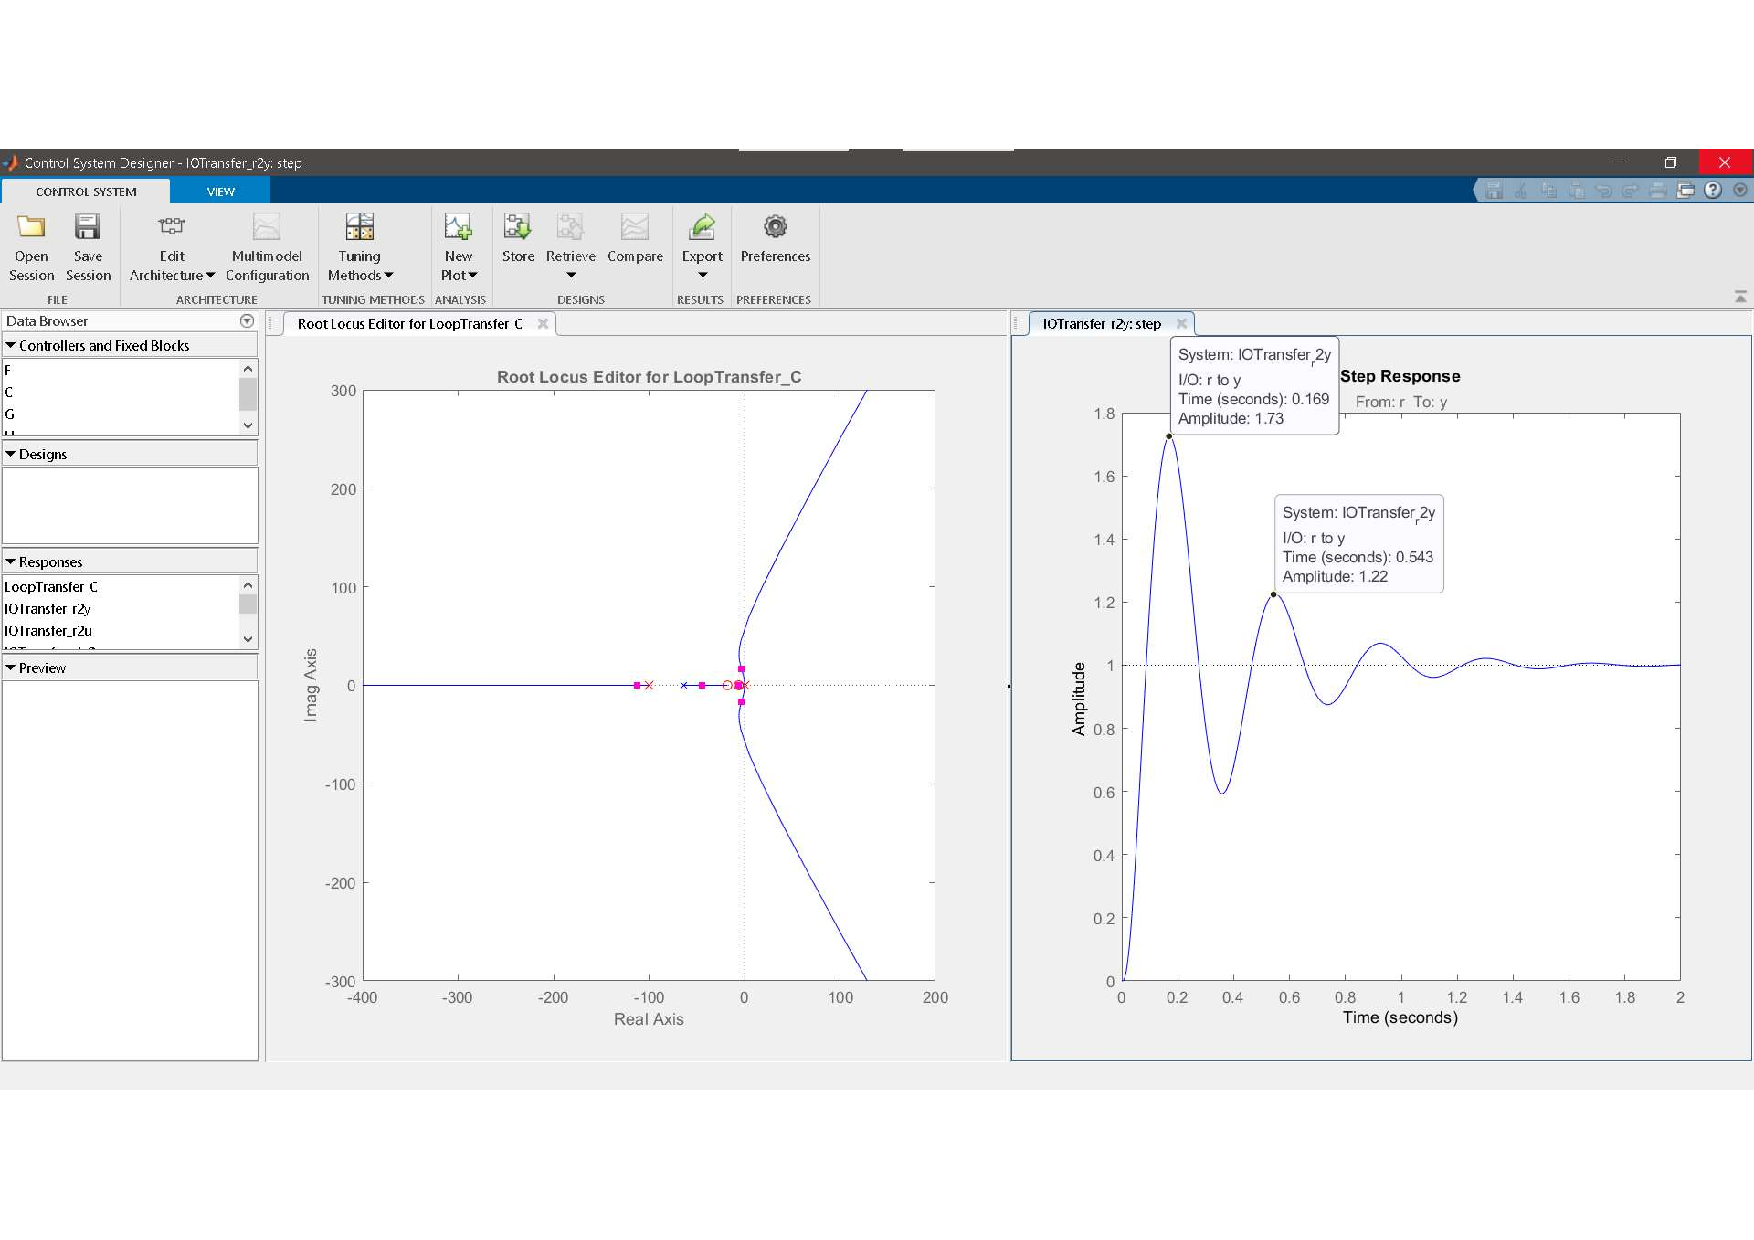
\includegraphics[clip, trim=0cm 3.5cm 0cm 2.8cm,scale=0.48]{images/figura 23.pdf}
  % izquierda,abajo,derecha,arriba
  \caption{Respuesta continua Ziegler-Nichols}
    \label{fig:figura 23}
\end{figure}
}
Calculamos la relación de sobreoscilación:\\
\begin{center}
  0.22/0.73 = 0.30 $\rightarrow$ 30\%
  \end{center}
  \vspace*{0.35em}
  \mkanscode{
\begin{figure}[H]
  \centering
  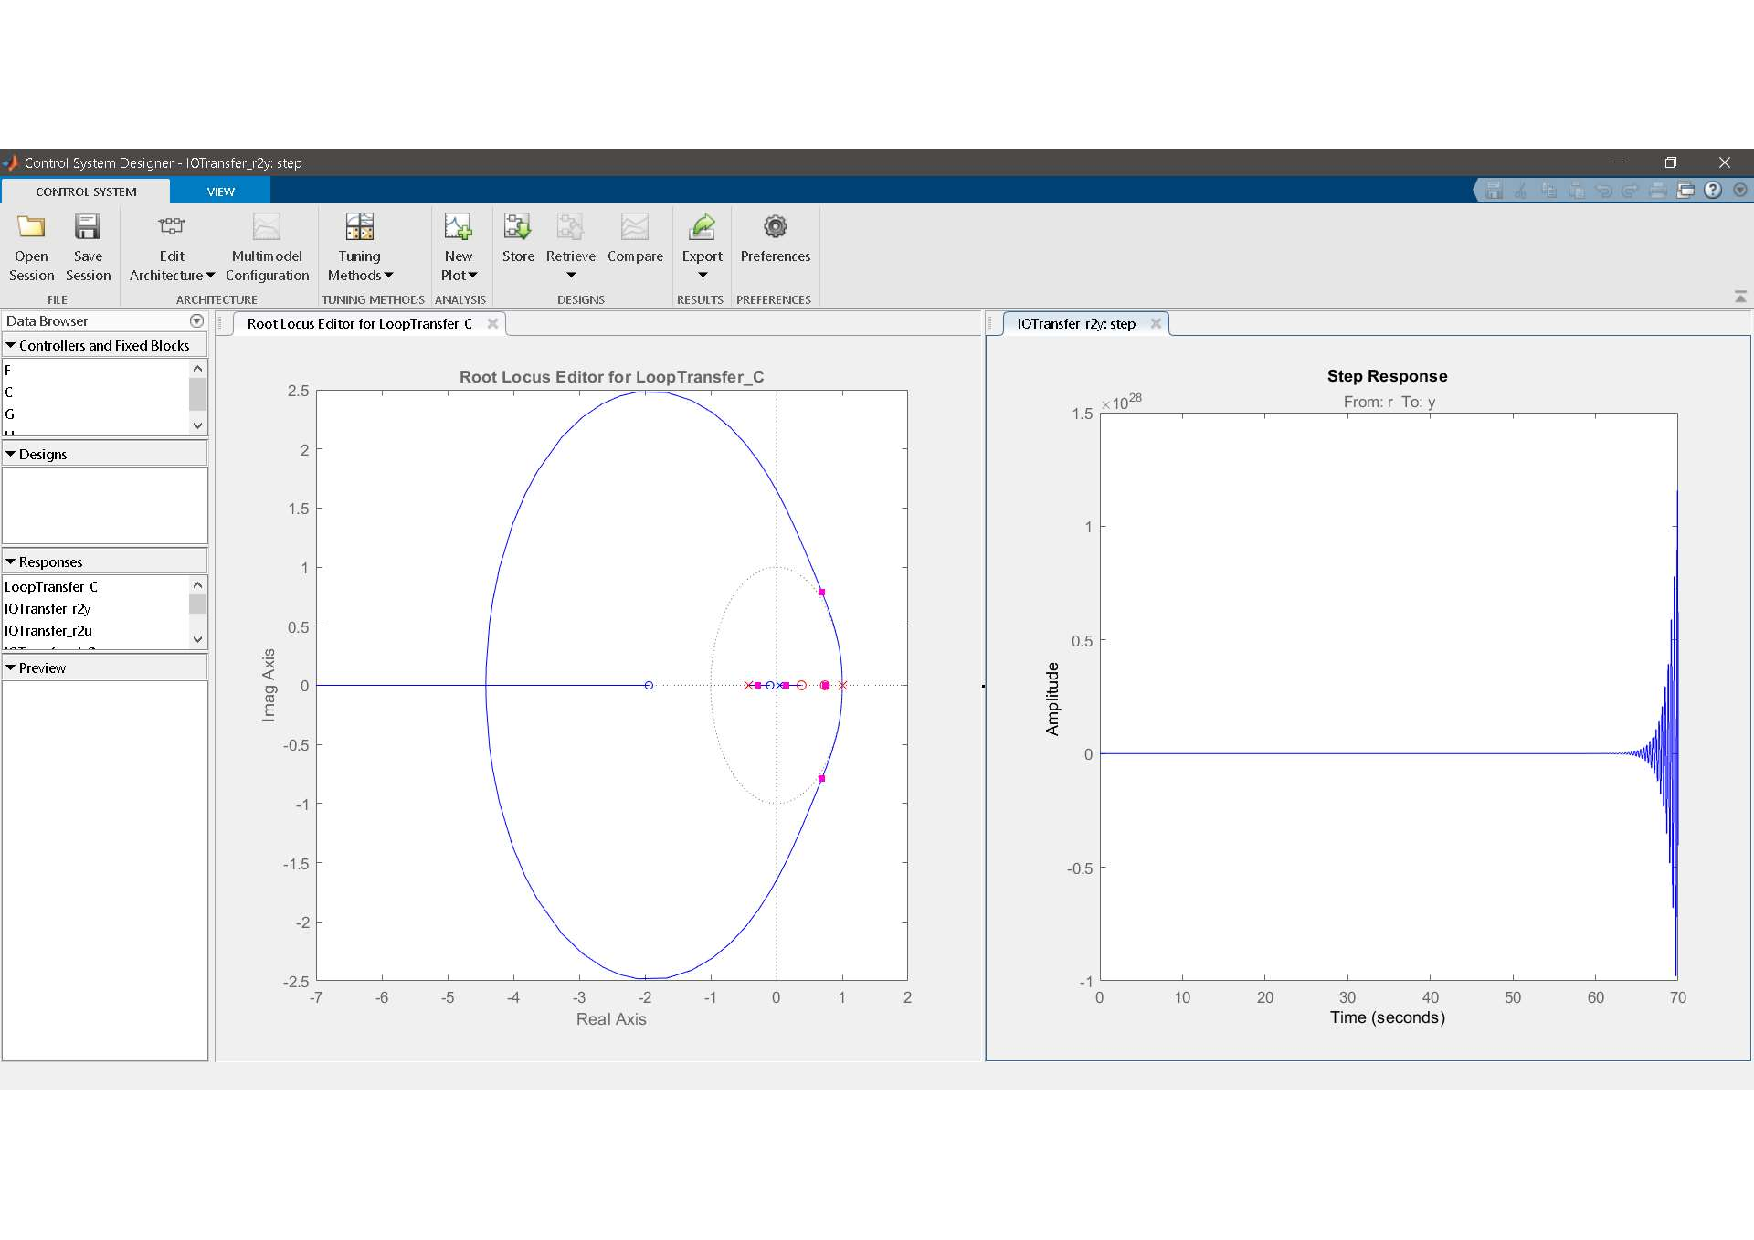
\includegraphics[clip, trim=0cm 3.5cm 0cm 2.8cm,scale=0.48]{images/figura 24.pdf}
  % izquierda,abajo,derecha,arriba
  \caption{Respuesta discretizada mediante el método Trapezoidal}
    \label{fig:figura 24}
\end{figure}
}
Mediante el método trapezoidal la discretización no es perfecta como
podemos observar, luego el método de discretización influye en la
respuesta lo que provoca que el sistema se vuelva inestable y que el
PID no cumpla su función.
  \end{tcolorbox}%